\documentclass[10pt,aspectratio=43]{beamer}

\usepackage{graphicx}
\usepackage{tikz}
\usepackage{xcolor}
\usepackage{caption}
\usepackage{subcaption}
\usepackage{bm}
\usetikzlibrary{calc} 
\usepackage{hyperref}
\hypersetup{
    colorlinks=true,
    linkcolor=blue,
    urlcolor=red
}
\usepackage{fontawesome5}
\usepackage{ulem}
\usepackage[dvipsnames]{xcolor}

\usetheme{MyStyle}   % loads beamerthemeMyStyle.sty
\setlength{\columnsep}{0pt}


%%%%%%%%%%%%%%%%%%%%%%%%%%%%%%%%%%%%%%%%%%
%%%%%%%%%%%%%%%%%%%%%%%%%%%%%%%%%%%%%%%%%%
%%%%%%%%%%%%%%%%%%%%%%%%%%%%%%%%%%%%%%%%%%

\title{Time reconstruction of saturated signals}
\newcommand{\eventname}{ALERT meeting}
\author{Felix Touchte Codjo}
\institute{IJCLab}
\date{\today}


\begin{document}

\begin{frame}[plain] % remove header, footer, barre de navigation
\titlepage
\end{frame}

%\begin{frame}{Outline}
%\tableofcontents
%\end{frame}

%\section{Intro}
\section{Updates}

\begin{frame}{Slope\_max as a good observable}
    \begin{itemize}
        \item For non-saturated signals, the ADC is proportional the slope (here the maximum of the derivative of the pulse)
        \item We can now predict the ADC value of saturated signals
            \[
                ADC_{corr} = \bm{f} (slope)
            \]
    \end{itemize}

    \centering
    \vspace{0.2cm}

    \begin{tabular}{cc}
        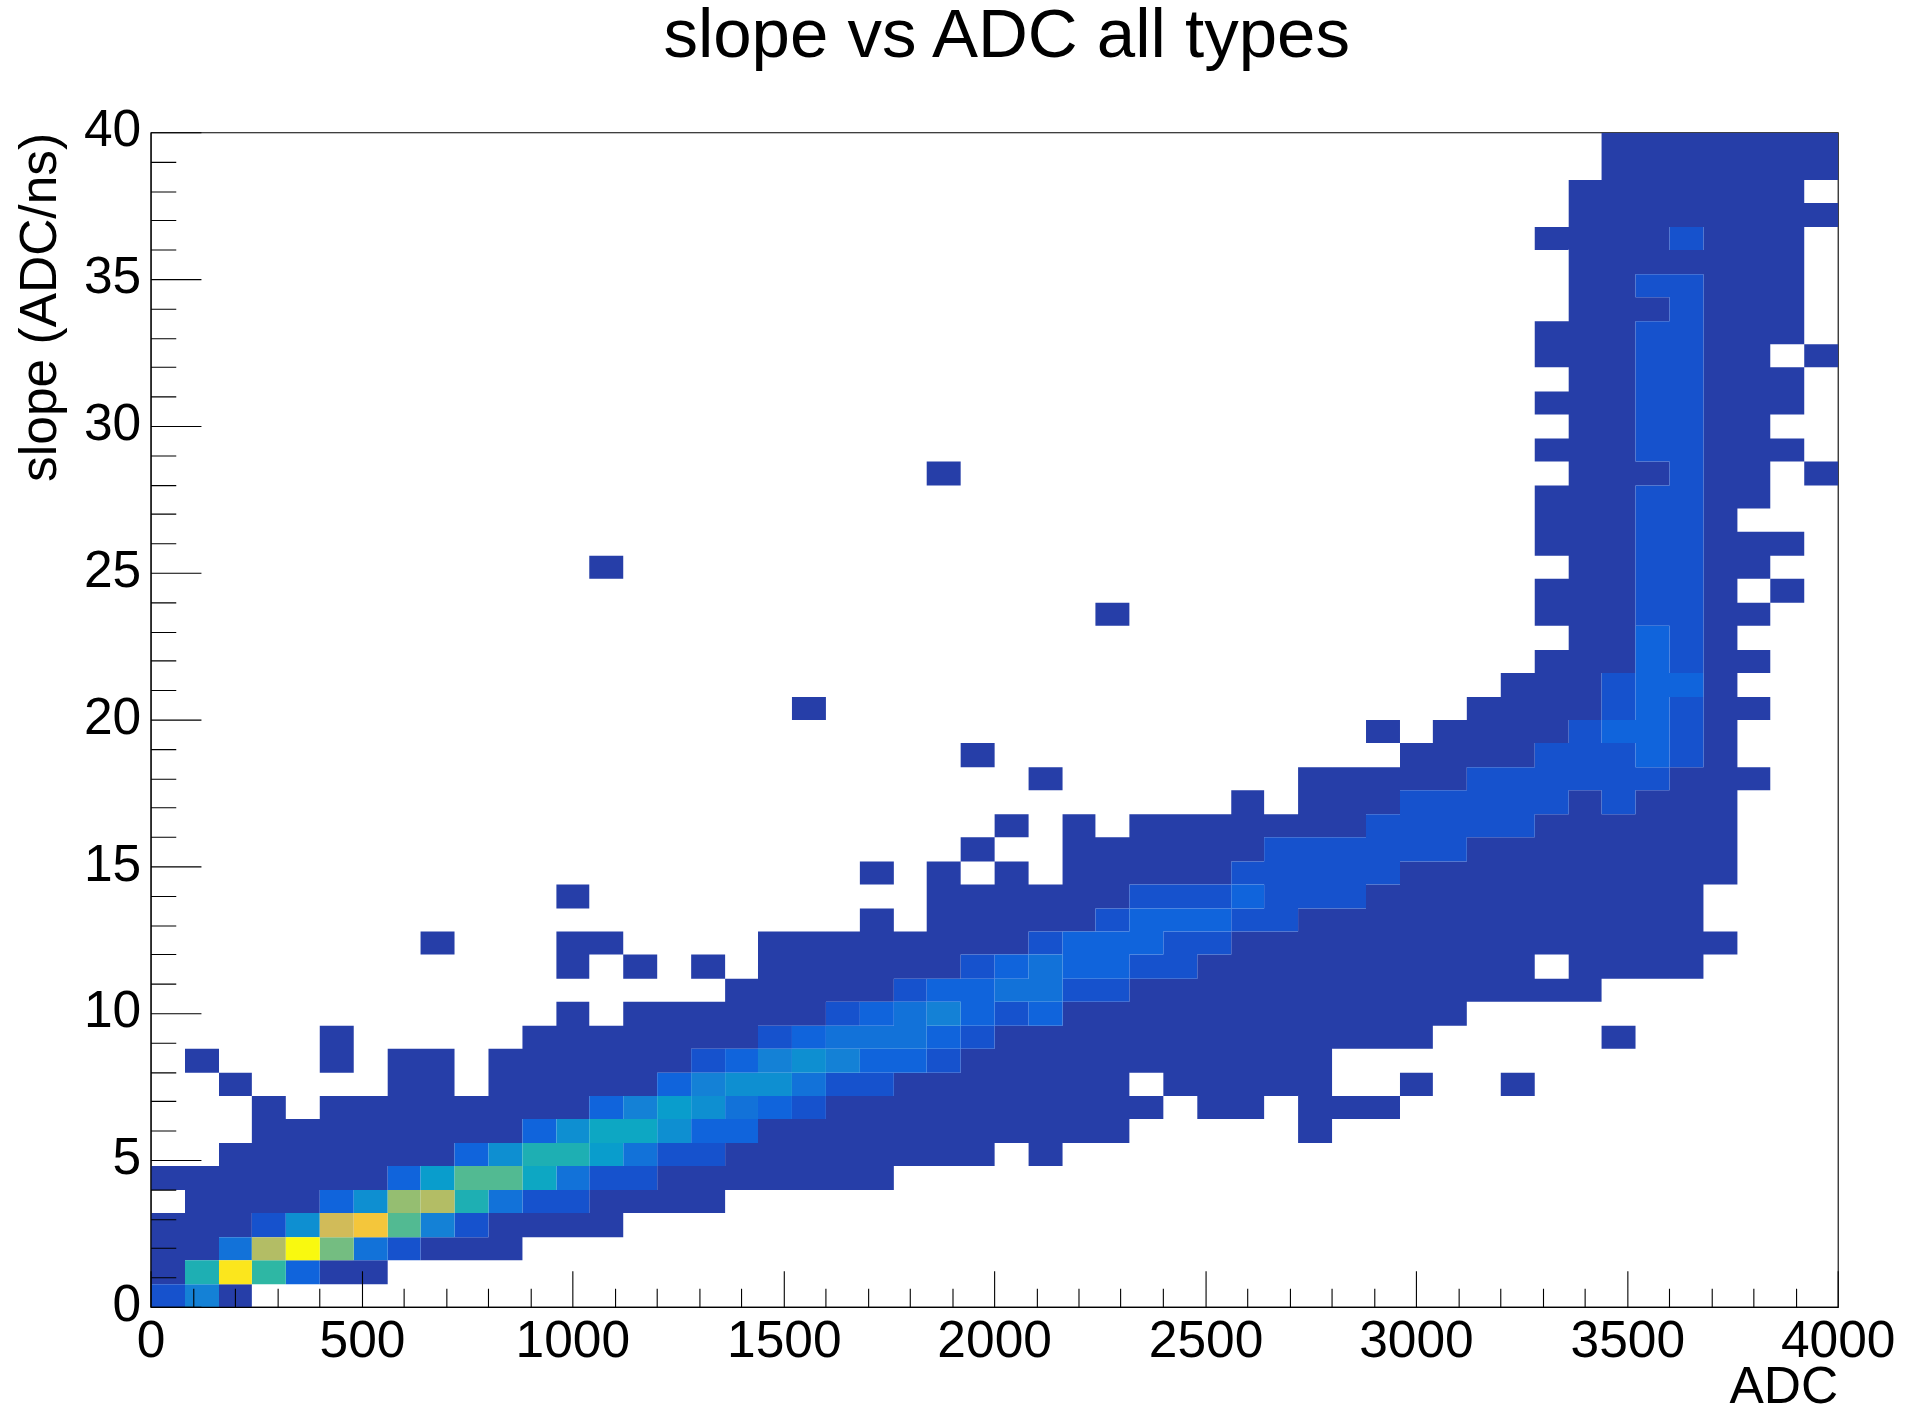
\includegraphics[width=0.42\linewidth]{figures/slope_vs_adc_all_wf.png} & 
            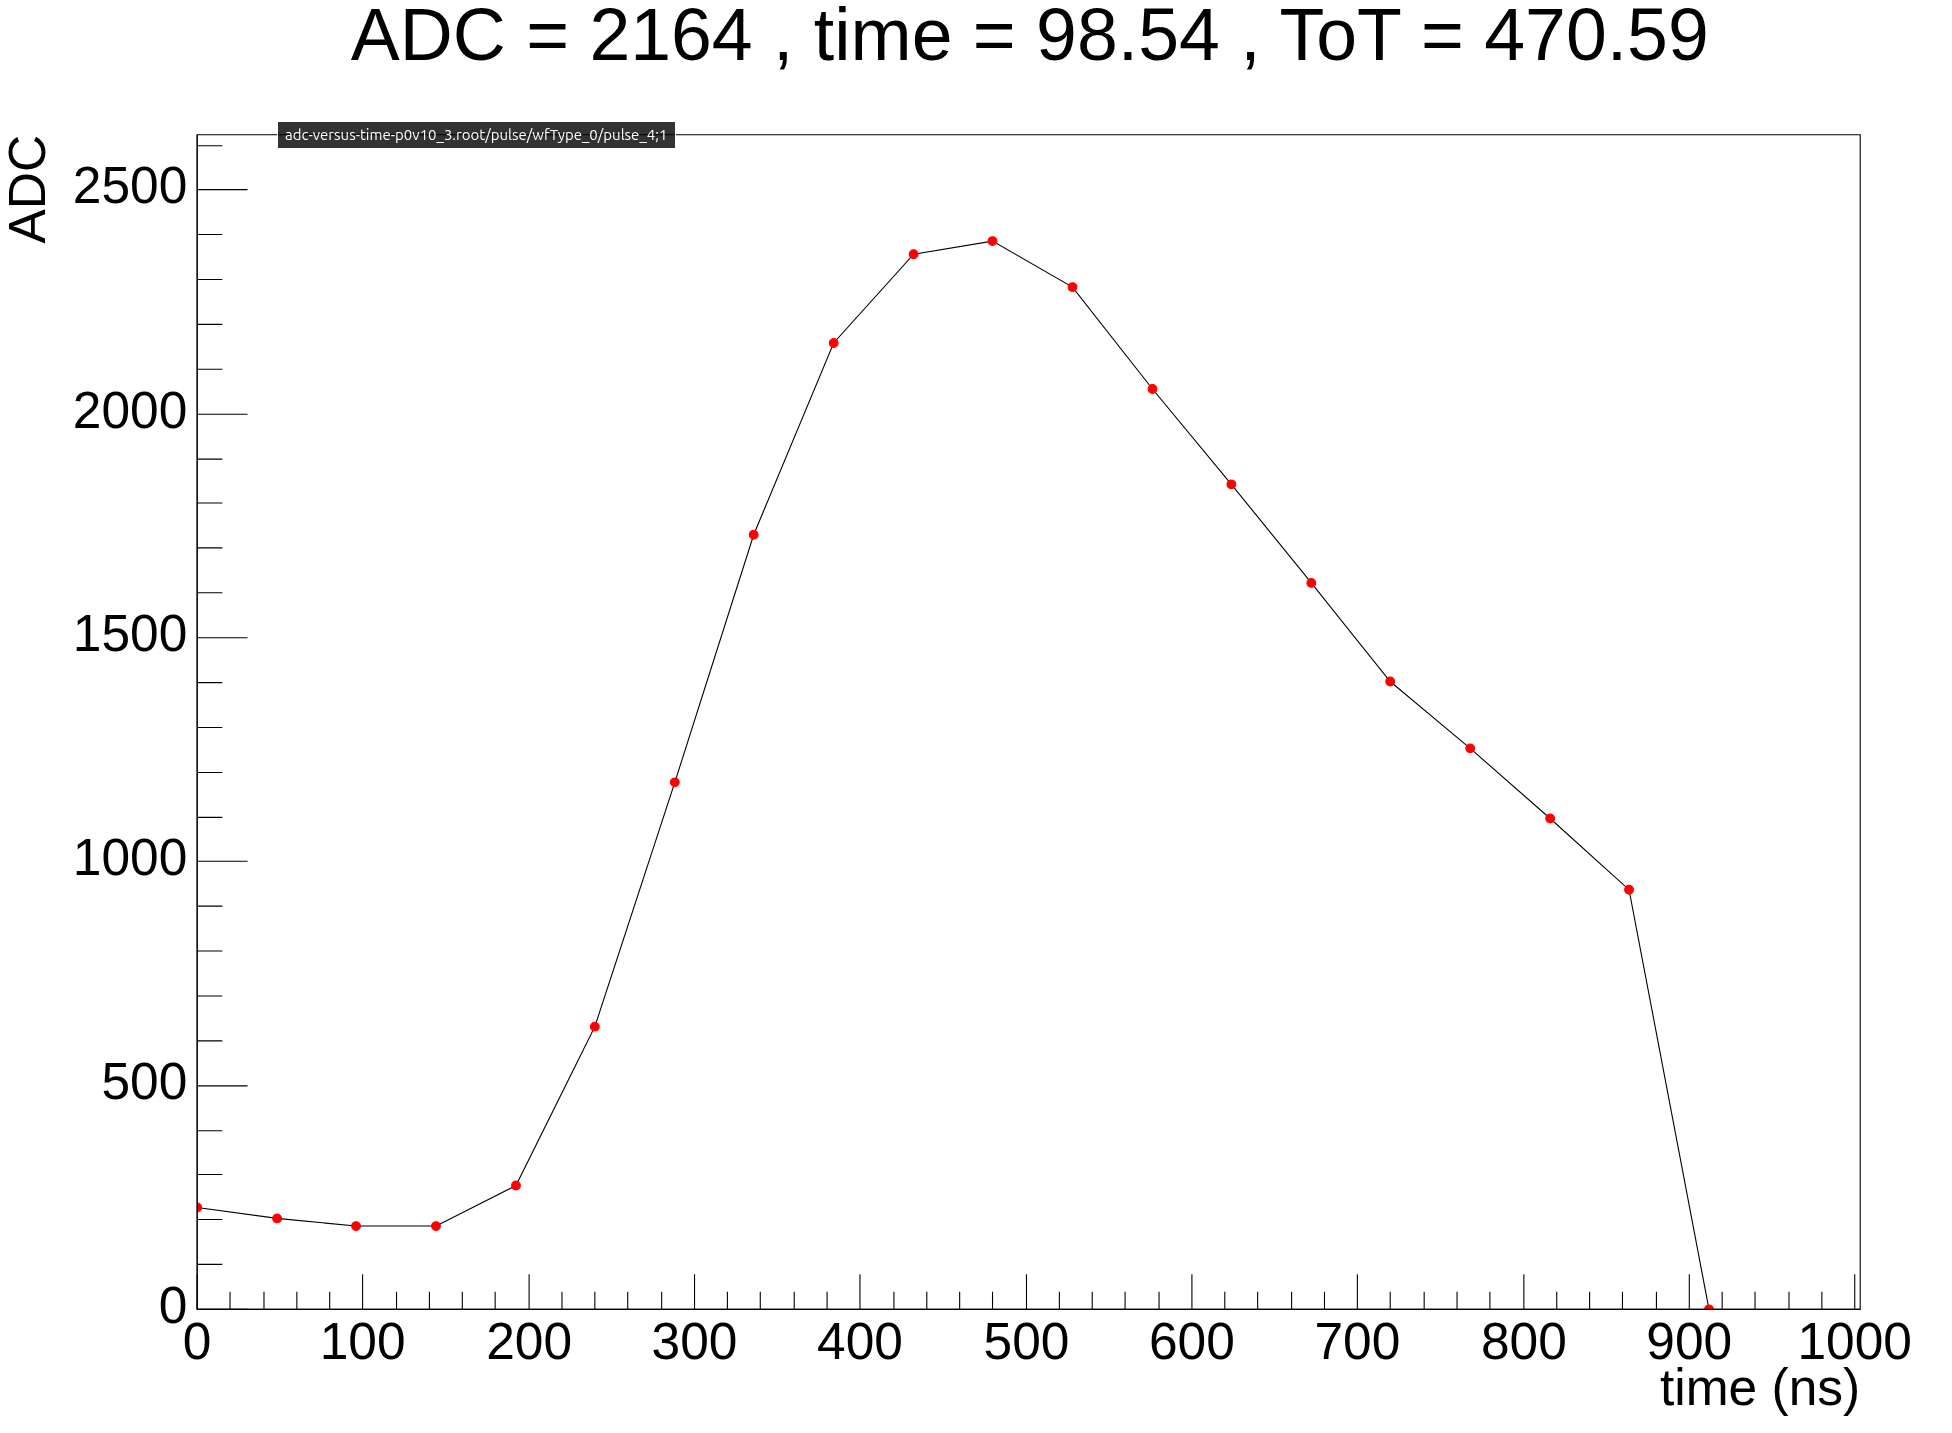
\includegraphics[width=0.42\linewidth]{figures/wfType0_pulse.png} \\
        %\includegraphics[width=0.4\linewidth]{figures/wfType1_pulse.png} & 
        %    \includegraphics[width=0.4\linewidth]{figures/wfType0_pulse_derivate.png} \\
    \end{tabular}

    % \begin{figure}
    %     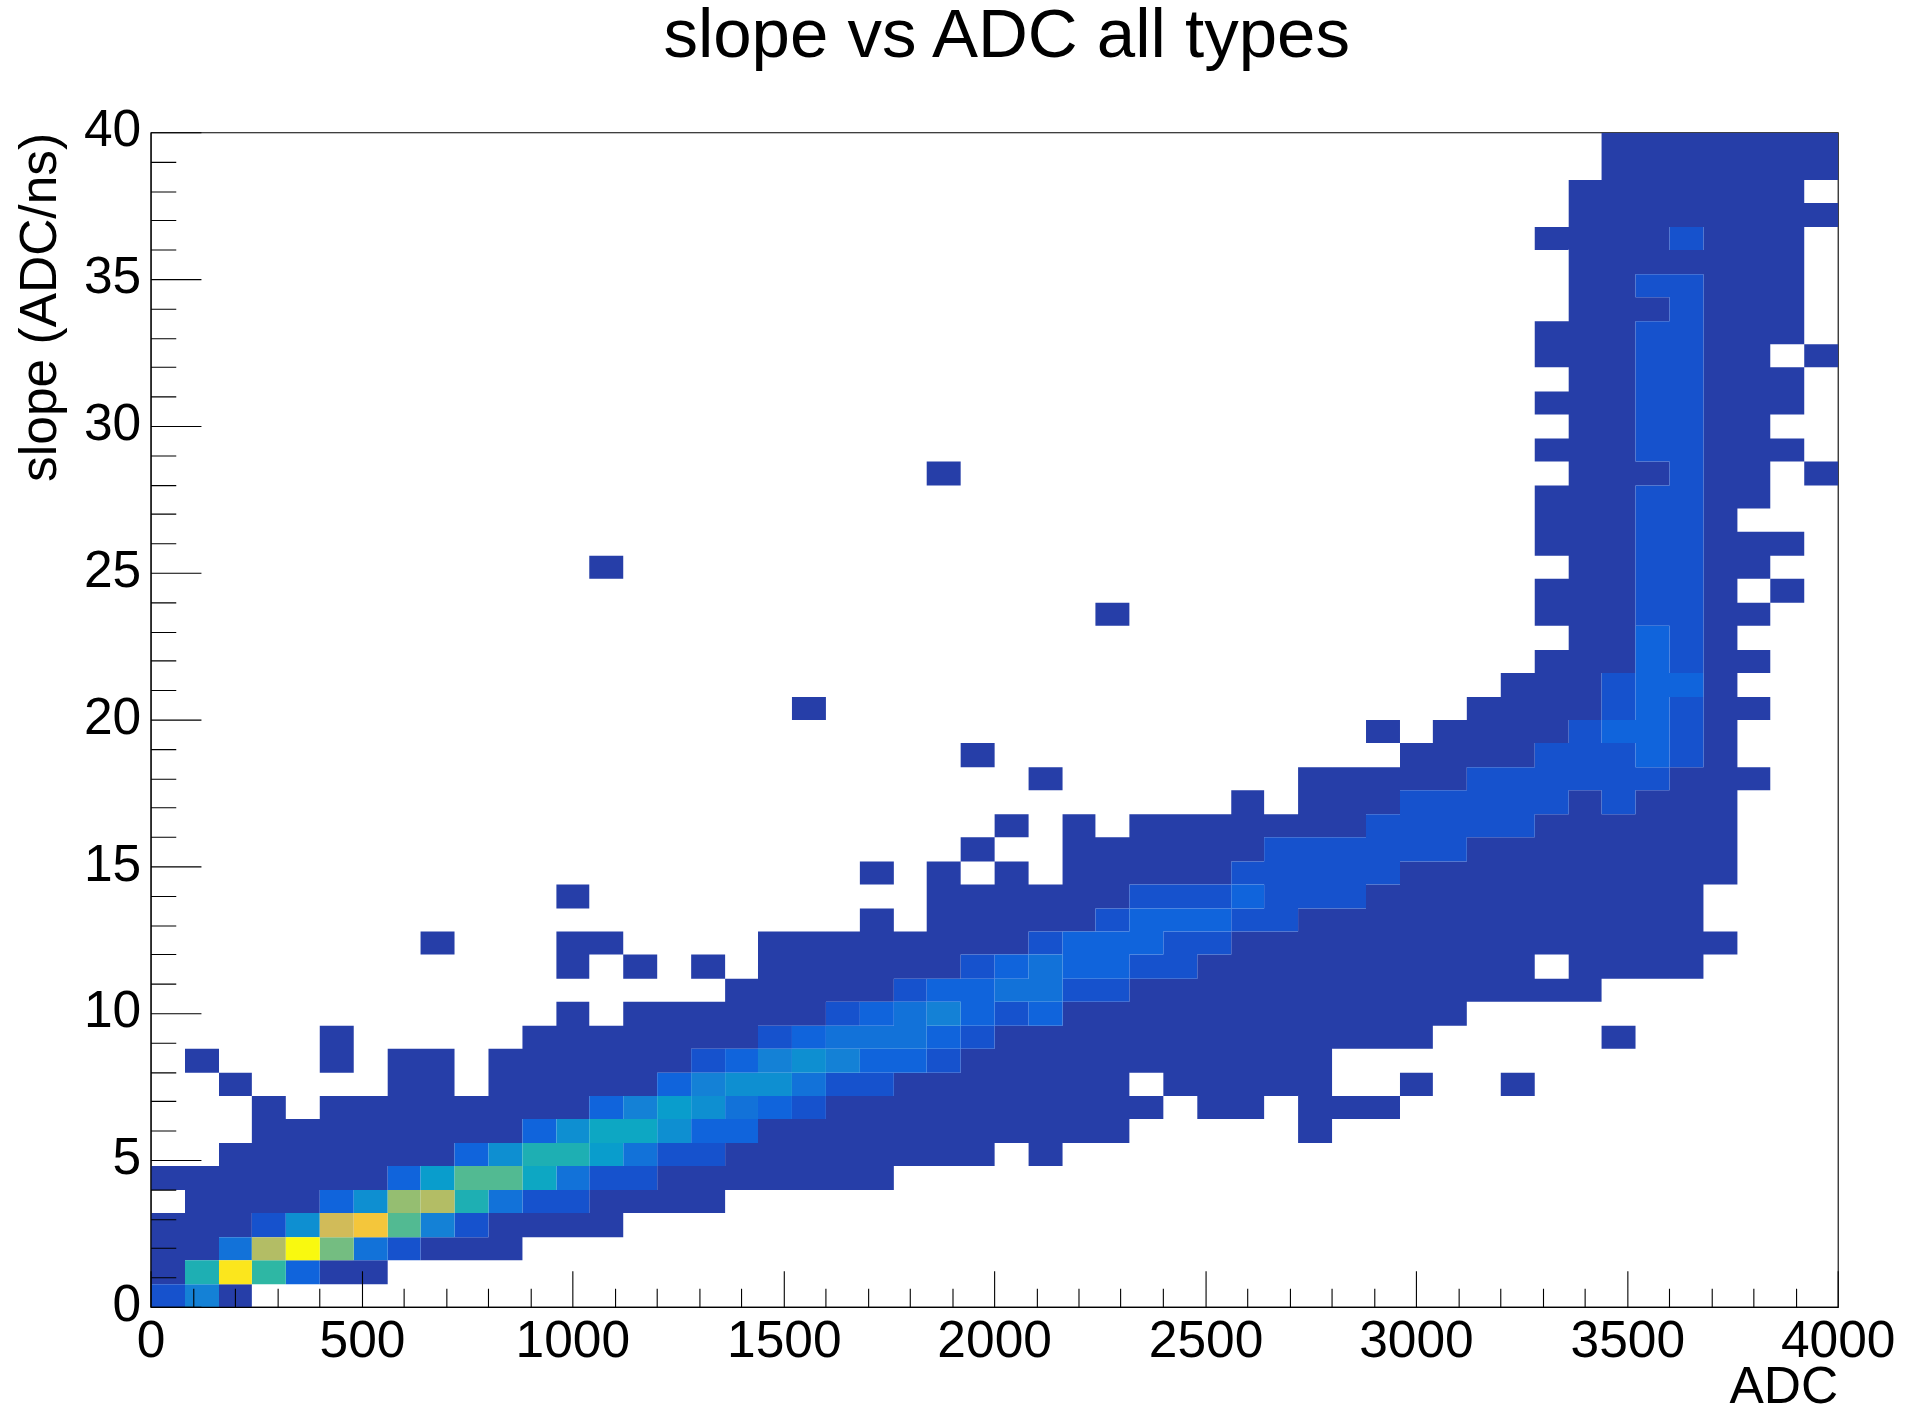
\includegraphics[width=0.6\linewidth]{figures/slope_vs_adc_all_wf.png}
    % \end{figure}

\end{frame}

\begin{frame}{Slope\_max as a good observable}
    \begin{itemize}
        \item Fit result
    \end{itemize}

    \centering
    %\vspace{0.2cm}

    \begin{figure}
        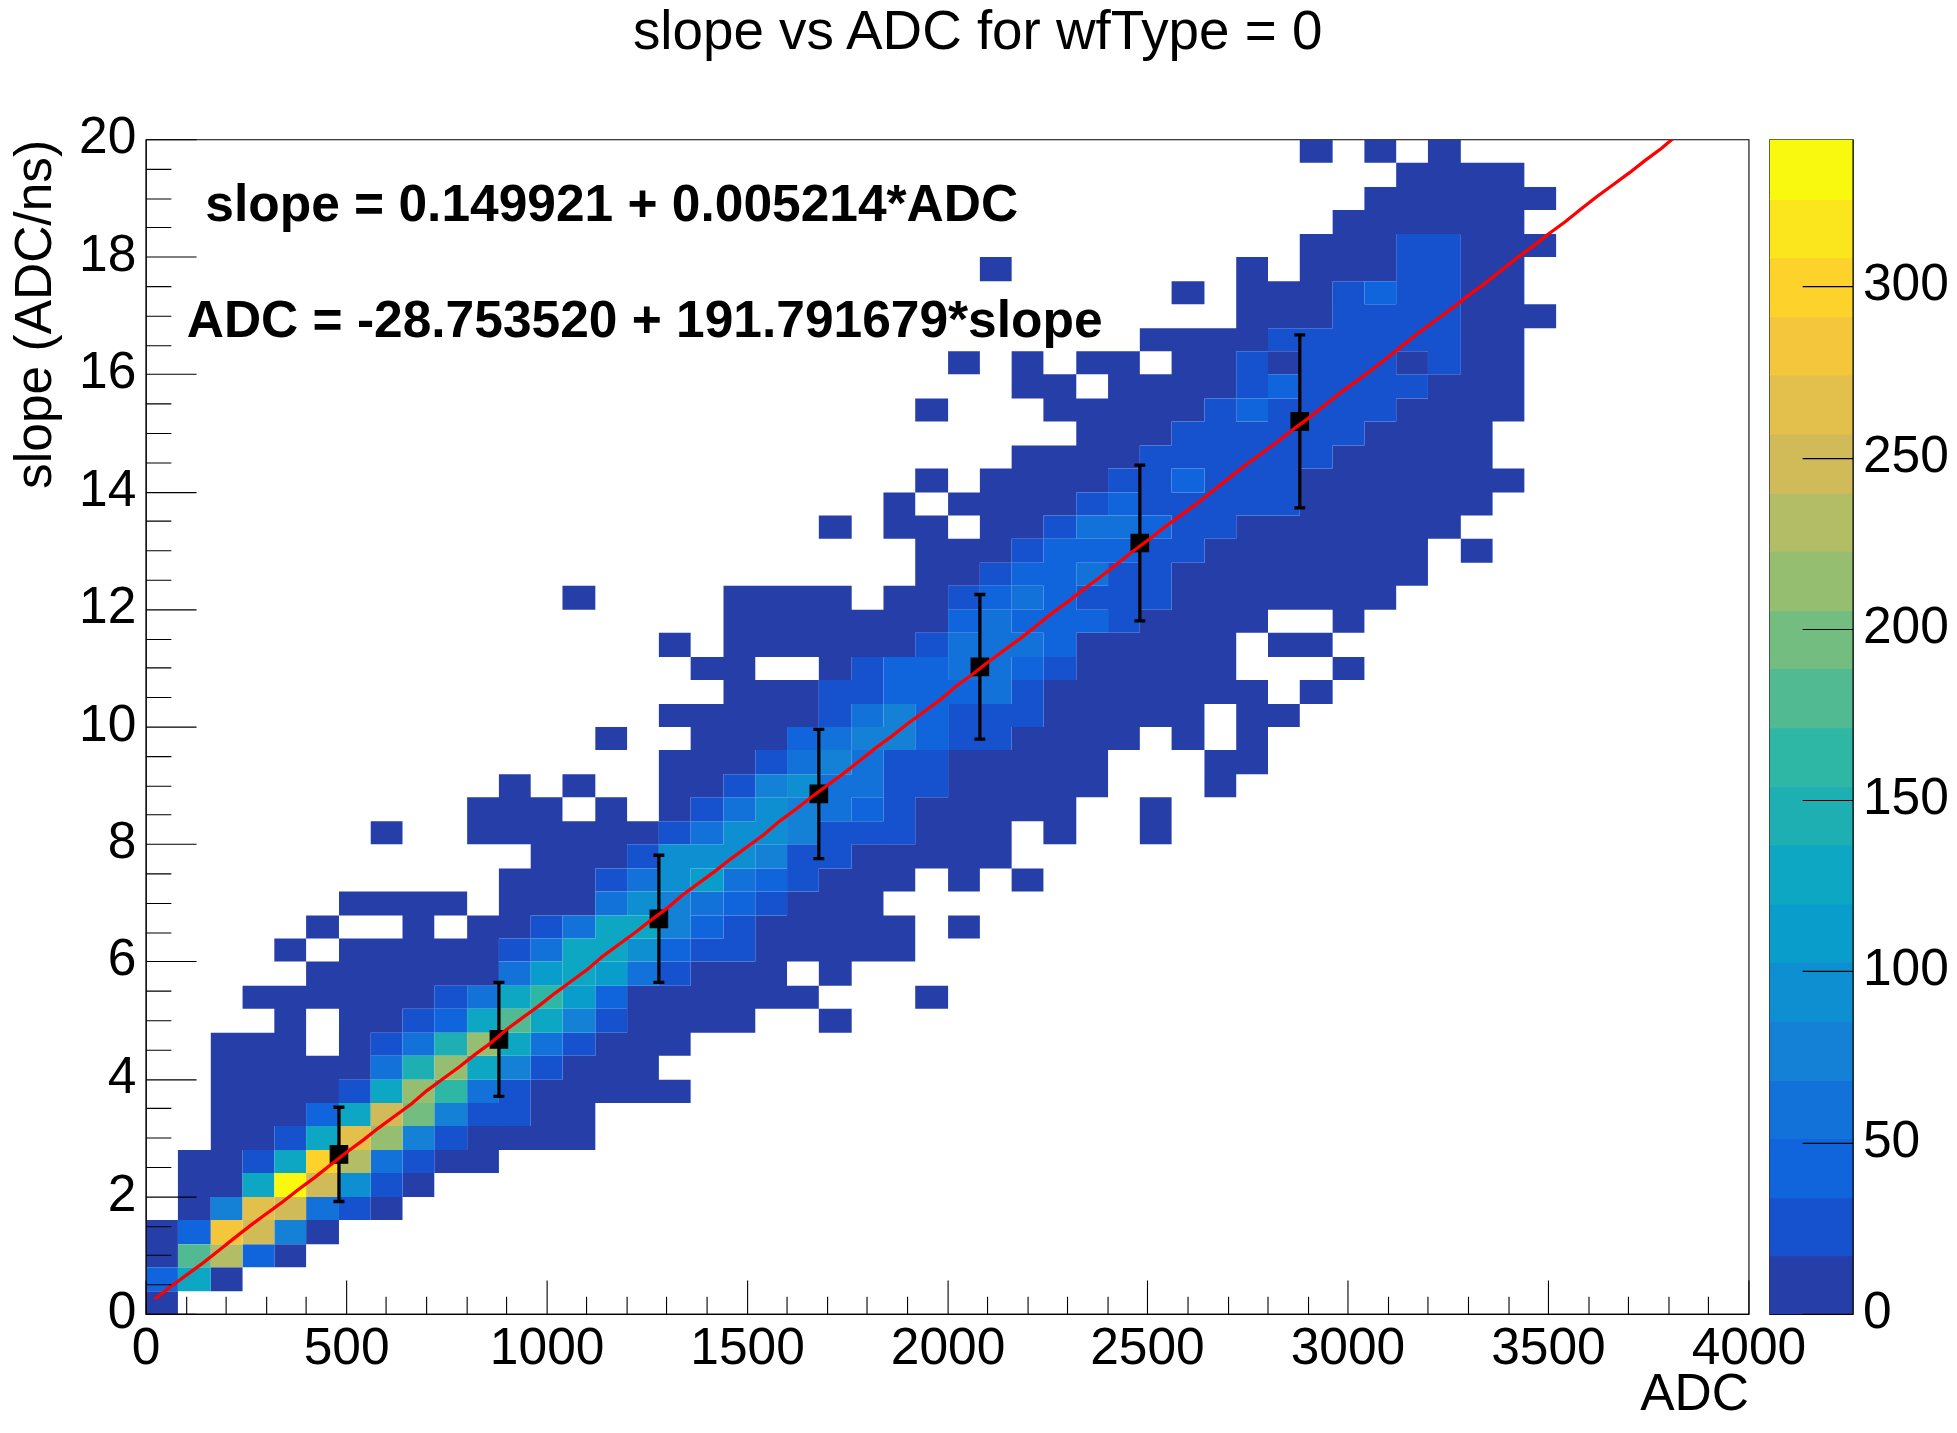
\includegraphics[width=0.5\linewidth]{figures/fit_adc_versus_slope.png}
    \end{figure}

    \begin{itemize}
        \item Next steps
        \begin{itemize}
            \item Recover the Time and ToT from $ADC_{corr}$
            \item Implement in coatjava
        \end{itemize}
    \end{itemize}

\end{frame}

\begin{frame}{Systematic bias and verification}
    \begin{itemize}
        \item Delta ADC for wfType 0
    \end{itemize}

    \centering
    \vspace{0.2cm}

    \begin{figure}
        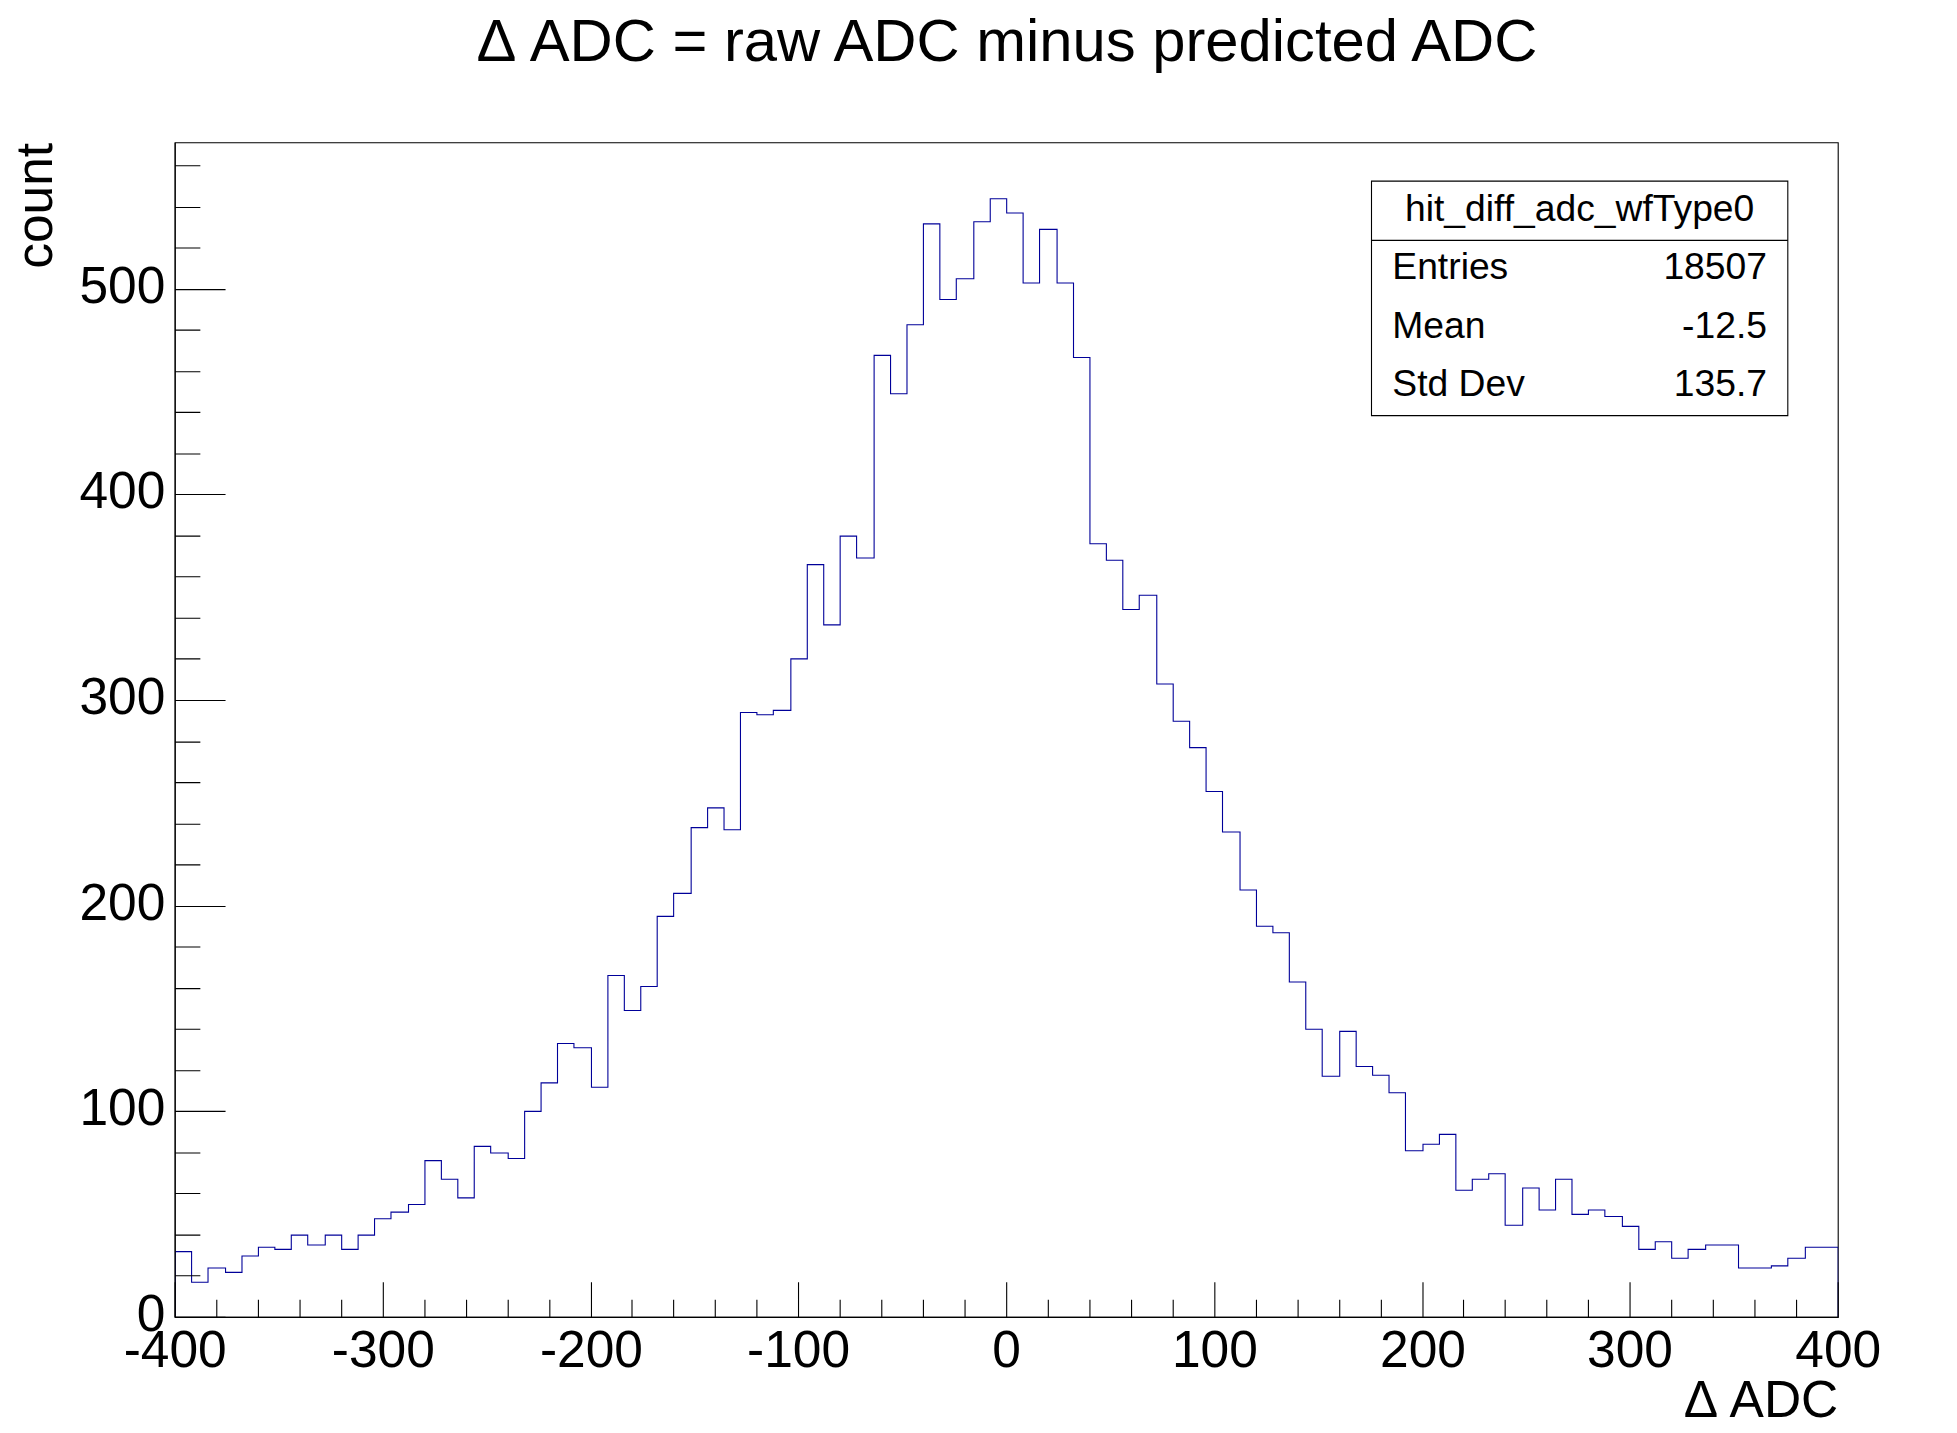
\includegraphics[width=0.6\linewidth]{figures/delta_adc_wfType0.png}
    \end{figure}

\end{frame}

\begin{frame}{Backup slides}
    \begin{itemize}
        \item Bias in the time reconstruction of saturated signals
        \item For such signals, the arrival time and the timeOverThreshold can be wrong
    \end{itemize}

    \centering
    \vspace{0.2cm}

    \begin{figure}
        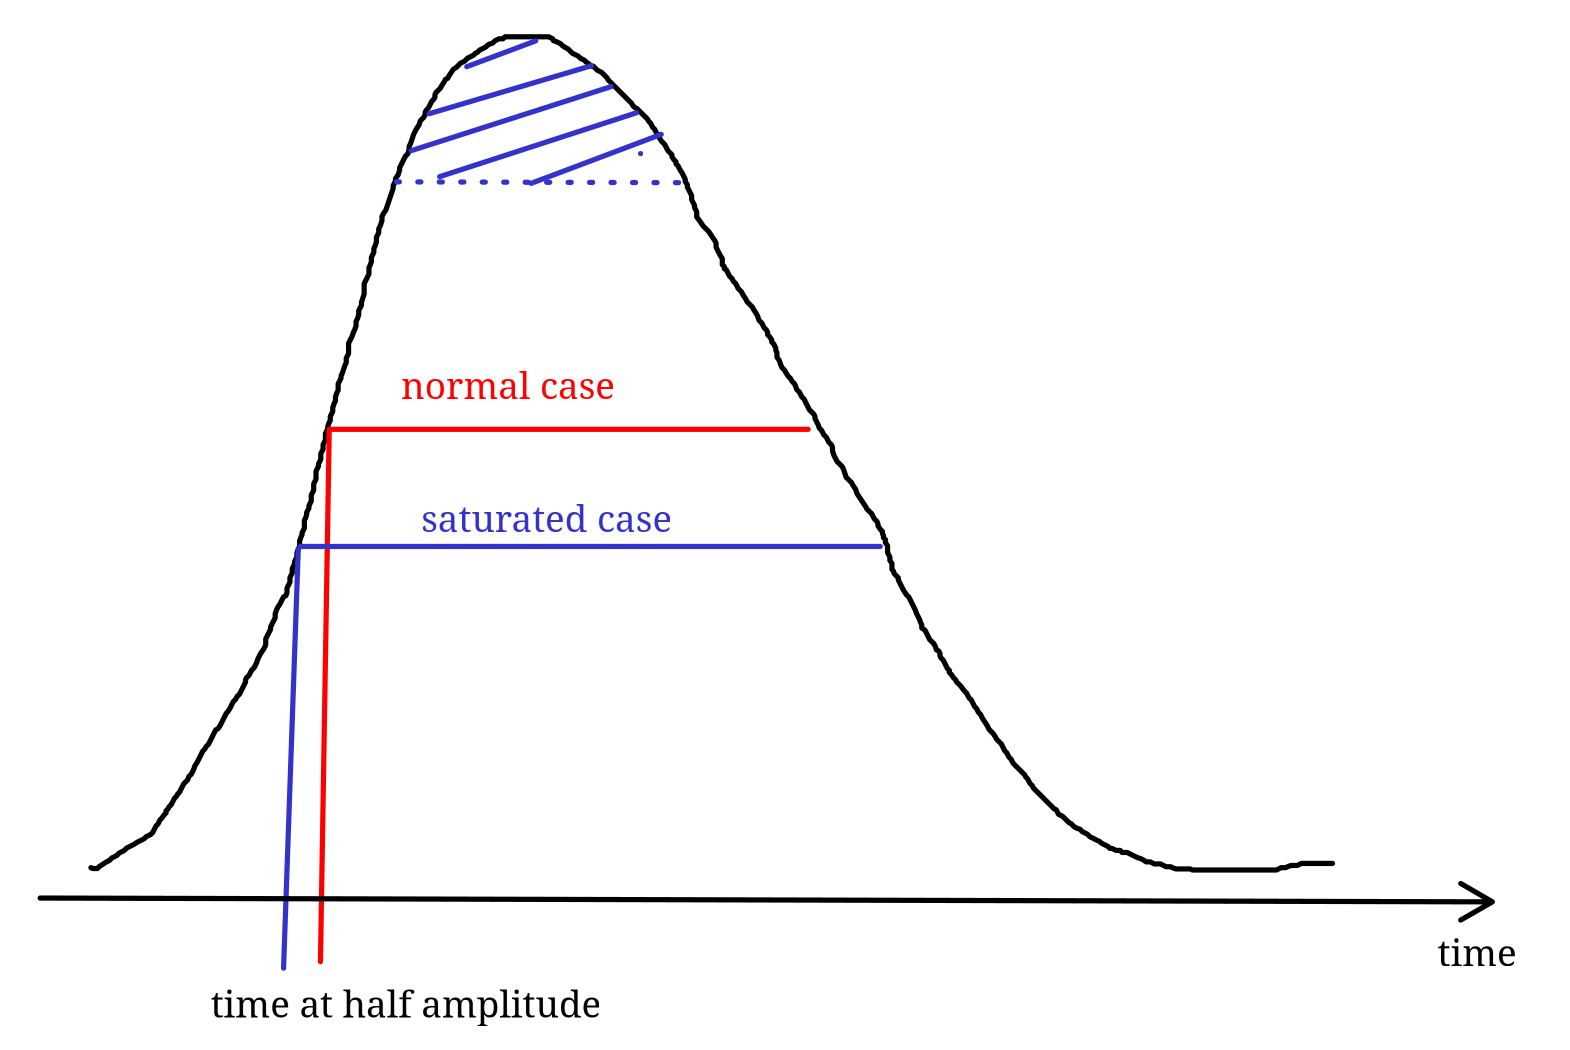
\includegraphics[width=0.65\linewidth]{figures/timewalk.png}
    \end{figure}

\end{frame}












\end{document}


